%%%%necessary for acta crystallographica

\section{Introduction}

\subsection{Motivation}
Since the first experimental demonstration of electron diffraction in 1928,
theory of dynamical diffraction has been developed~\cite{Bethe1928,CowleyBook}.
Besides, multiple scattering~\cite{Korringa1947,Kohn1954,Korringa1994,Dederichs1971}
has also extensively been studied in solid state physics over the 20th century.
In fact, even at very high electron energies commonly used in modern transmission electron
microscopes, the electron-atom interaction is very strong and the the kinematic
theory of diffraction is not theoretically valid for crystals thicker than a
few nm\cite{GlaeserDowning1993,SubramanianSpence2015}. In practice, crystal
growth cannot be controlled to such a degree of accuracy and nano-crystals
of organic compounds are usually on the order of tens to hundreads of nanometers.
This is known as a challenging aspect of high energy electron diffraction (HEED) as it
should significantly complicate the structure determination process.
However, successfull structure determination based on the standard kinematic
theory used in X-ray diffraction have regularly been demonstrated over the
past 10 years\cite{Nannenga2014,Nannenga2019} suggesting that dynamical diffraction may
not affect the diffraction intensities as much as the theory suggests.
Although, dynamical refinement based structure determination~\cite{Palatinus2013} usually
leads to better intensity predictions~\cite{Gemmi2019b}, the agreement
between theory and experiment is still significantly worse than those obtained
for X-rays~\cite{Oleynikov2007}. It is therefore crucial to develop more
accurate models of electron diffraction by crystals.

\subsection{state of the art}
The multislice(MS)~\cite{CowleyMoodie1957} and Blochwave(BW)~\cite{Bethe1928}
approaches are the most popular methods for simulating scattering of high energy
electrons in crystals.
The MS is particularly well suited for solving large structures as it involves
successive convolutions which can be very efficiently computed with the Fast
Fourier Transform(FFT)~\cite{Ishizuka1977}. To avoid aliasing transverse periodic
boundary conditions must be met which is only possible for orthorombic
structures in zone axis orientations. Although small beam tilt can also be
used~\cite{Ishizuka1982,ChenDyck1997}, simluations with arbitrary orientations
must be performed by simulating a full crystal with added zero padding. This
can quickly become computationnally challenging.

On the other hand, BW method can simulate small structures in any arbitrary
orientations. Although some efficient implementation~\cite{Zuo1995} can simulate
moderately large structures, BW cannot be applied to large structures due to
the unfavorable scaling behaviour of the matrix diagonalization involved.
Non periodic structures, defects and solvent scattering cannot be modelled either.

Both approach can handle coherent inelastic scattering through the use of
a imaginary part of the potential. This however does not account for the
loss of coherency induced by inelastic scattering which may have dramatic
impact on the dynamical diffraction~\cite{Latychevskaia2019}.


\subsection{Contribution and outline}

The purpose of this paper is to propose an alternative real space approach
to the scattering of fast electrons by light-atom structures based on
the T-matrix formalism.
The T-matrix has been extensively applied to various areas of physics including
electromagnetics~\cite{Hamid1990,Hamid1990_b,Eremin1995}, optics~\cite{Moine2005}
and acoustics~\cite{Silva2012,Godin2011}.
Although not computationnally competitive with multislice
for large systems, this approach provides an exact solution to Schr{\"o}dinger's
equation for an assemble of spherically symmetric effective atomic potentials in
the independent atom model (IAM).
An intuitive understanding of multiple scattering in the forward scattering
approximation is presented and compared with existing intepretations.
The validity of the forward scattering approximation and the phase grating
approximation used by multislice are then discussed.
Conclusions are drawn and extensions of this approach to account for incoherent
inelastic scattering are outlined.





%%%%%%%%%%%%%%%%%%%%%%%%%%%%%%%%%%%%%%%%%%%%%%%%%%%%%%%%%%%%%%%%%%%%%%%%%
%%%%%%%%%%%%%%%%%%%%%%%%%%%%%%%%%%%%%%%%%%%%%%%%%%%%%%%%%%%%%%%%%%%%%%%%%
%%%%%%%%%%%%%%%%%%%%%%%%%%%%%%%%%%%%%%%%%%%%%%%%%%%%%%%%%%%%%%%%%%%%%%%%%
%%%% Theory
%%%%%%%%%%%%%%%%%%%%%%%%%%%%%%%%%%%%%%%%%%%%%%%%%%%%%%%%%%%%%%%%%%%%%%%%%
%%%%%%%%%%%%%%%%%%%%%%%%%%%%%%%%%%%%%%%%%%%%%%%%%%%%%%%%%%%%%%%%%%%%%%%%%
%%%%%%%%%%%%%%%%%%%%%%%%%%%%%%%%%%%%%%%%%%%%%%%%%%%%%%%%%%%%%%%%%%%%%%%%%
\section{Theory}

The problem of the scattering of fast electrons by an assembly of atoms is
found by solving Schr{\"o}odinger's equation :
%
\begin{equation}\label{eq:schro}
  \left[-\frac{\hbar^2}{2m_e}\grad_{\bb r}^2 - eV(\bb r) \right] \Psi = E\Psi
\end{equation}
%
where $\hbar$ is plank's constant, $m_e$ the mass of the electron,
$e$ the elementary charge, $V(\bb r)$ is the spatially varying electrostatic
potential created by the atoms and $E$ the energy of the incident electrons.
The wave function is sought as a sum of an incident wave $\Psi^{(i)}$
and a scattered wave $\Psi^{(s)}$.

\subsection{T-matrix formulation}

\begin{figure}
  \centering
  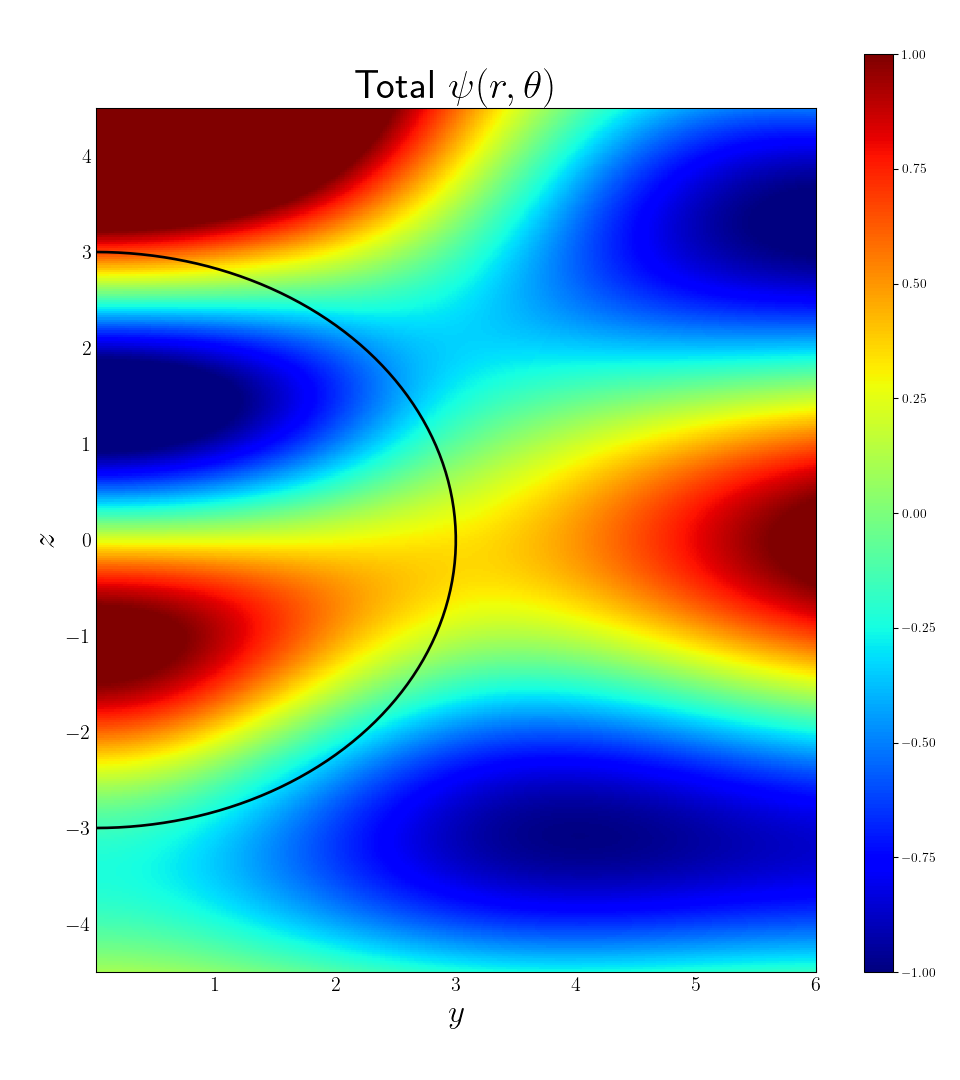
\includegraphics[height=0.25\textheight]{figures/Tmatrix.png}
\caption{The problem solved by the T-matrix}\label{fig:Tmatrix}
\end{figure}

In its standard form, the T-matrix solves for the case where the electrostatic
potential is uniform constant inside non overlapping spheres and the
incident wave is described by a plane wave of wavenumber $k_0=2\pi/\lambda$
(optics convention).
The setup shown in figure~\ref{fig:Tmatrix}.
The formulation is well established and the theory is outlined for the purpose
of introducing the forward multiple scattering approximation picture.

In each domain, the problem is reduced to Helmholtz's equation
in spherical coordinates  :
%
\begin{eqnarray*}
  \grad_{\bb r_p}^2\Psi + k_p^2 \Psi &=& 0\\
  k_p &=& k_0n_p\\
  k_0 &=& \sqrt{\frac{2m_eE}{\hbar^2}}\\
  n_p &=& \sqrt{1+\frac{V_p}{E}}
\end{eqnarray*}
%
where $V_p\ge 0$ is the constant attractive potential inside sphere $p$ of radius
$a_p$ centered at $\bb d_p$, $k_p$ the wave number inside the sphere and $n_p$
can be referred to as the refractive index by analogy with optics.
The scattered wave function inside and outside of sphere $p$ can then be expressed
as :
%
\begin{eqnarray*}
  \Psi_p^{(in )}(\bb r_p) &=& \sum_{l=0}^{\infty}j_l(k_pr_p)\sum_{m=-l}^{m=l}a_{p;lm}Y_l^m(\theta_p,\phi_p)\\
  \Psi_p^{(out)}(\bb r_p) &=& \sum_{l=0}^{\infty}\hl(k_0r_p)\sum_{m=-l}^{m=l}b_{p;lm}Y_l^m(\theta_p,\phi_p)\\
\end{eqnarray*}
%
where $p=1..N$,
$j_l$ and $\hl$ are the spherical Bessel and Hankel functions of the first
kind, $Y_l^m$ are the spherical harmonics or order $l$ and azimuthal order $m$.
Note that these equations are expressed in the reference frame of each
sphere $p$ hence the use of variable $\bb r_p$.

The unknown coefficients $a_{p;lm}$, $b_{p;lm}$ are found by imposing the
continuity of the wave function and its radial derivative at the surface of each
sphere $p$ :
%
\begin{eqnarray*}
      \Big(\sum_{q=1}^N \Psi_q^{(out)}+\Psi^{(i)}\Big)\big|_{r_p=a_p}
  &=& \Big(\Psi_p^{(in)}\Big)\big|_{r_p=a_p} \\
      \dP_{r_p}\Big(\sum_{q=1}^N \Psi_q^{(out)}+\Psi^{(i)}\Big)\big|_{r_p=a_p}
  &=& \dP_{r_p}\Big(\Psi_p^{(in)}\Big)\big|_{r_p=a_p} \\
\end{eqnarray*}
%
where $f^{(i)}$ is the incident electron wavefunction and $a_p$ the
radius of sphere $p$.

Using the orthogonality of the spherical harmonics
% $\int_{\Omega} Y_{l}^{m}Y_{l'}^{m'*}d\Omega=\delta_{l,l'}\delta_{m,m'}$,
the following linear system yields the unknown coefficients :
%
\begin{eqnarray}
  a_{p;lm} &=& u_{p;l}c_{lm} + u_{p;l}\sum_{q\neq p}^{N} \nonumber\\
    &&~~\sum_{\nu=0}^{\infty}\sum_{\mu=-\nu}^{\mu=\nu}
      a_{\nu,\mu;l,m}^{(out-in)}(\bb d_{pq})b_{q;\nu\mu}\label{eq:aplm}\\
  b_{p;lm} &=& v_{p;l}c_{lm} + v_{p;l} \sum_{q\neq p}^{N}\nonumber\\
    &&~~\sum_{\nu=0}^{\infty}\sum_{\mu=-\nu}^{\mu=\nu}
      a_{\nu,\mu;l,m}^{(out-in)}(\bb d_{pq})b_{q;\nu\mu}\label{eq:bplm}\\\nonumber
\end{eqnarray}
%
where
the translational addition theorem\cite{Dufva2008} has been
used to express the field scattered by sphere $q$ in the reference
frame of sphere $p$, formally written as $f_q^{(out)}(\bb r_p)$.
This operation involves the coupling coefficients
$a_{\nu,\mu;l,m}^{(out-in)}(\bb d_{pq})$
where $\bb d_{pq}=\bb d_q-\bb d_p$.
%
% \begin{eqnarray*}
%   d_{pq}  &=& ||\bb d_q-\bb d_p|| \\
%   \theta_{pq} &=& \arccos\left(\frac{z_q-z_p}{d_{pq} }\right)\\
%   \phi_{pq}   &=& \arctan\left(\frac{y_q-y_p}{x_q-x_p}\right)\\
% \end{eqnarray*}
%

The coefficient $c_{lm}$ are related to the incident wave.
In the case of a plane wave $e^{j\bb k_0\cdot\bb r}$, $j=\sqrt{-1}$,
the addition theorem is used to expand the plane wave on
the family basis os Spherical Bessel soluions :
\begin{eqnarray*}
  c_{lm}  &=& 4\pi j^l Y_l^{m*}\left(\alpha_i,\phi_a\right)e_p\\
  e_p     &=& e^{jk_0d_p\zeta_p}\\
  \zeta_p &=& \sin(\Theta_p)\sin(\Phi_p)\sin(\alpha_i)+
              \cos(\Theta_p)\cos(\alpha_i)\\
\end{eqnarray*}
%
where $d_p,\Theta_p,\Phi_p$ being the spherical coordinates of the
centre of sphere $p$ in the global coordinate system,
$0\le\alpha_i\le\pi$ is the angle of incidence with respect to
the $\bb e_z$ axis, $\phi_i=\pi/2$ since the propagation is in the $(y,z)$
plane and $e_p$ is the phase offset at sphere $p$.
The different notations as illustrated on figure~\ref{fig:Tmatrix}.

The coefficients $u_{p;l}$ and $v_{p;l}$ are expressed as :
\begin{eqnarray*}
  u_{p;l} &=& \frac{h_l^{'}(k_0a_p)j_l(k_0a_p) - h_l(k_0a_p)j_l(k_0a_p)^{'}}
    {j_l(k_pa_p)h_l^{'}(k_0a_p)-n_pj_l^{'}(k_pad_p)h_l(k_0a_p)} \\
  v_{p;l} &=& \frac{n_pj_l^{'}(k_pa_p)j_l(k_0a_p) - j_l(k_pa_p)j_l^{'}(k_0a_p)}
    {j_l(k_pa_p)h_l^{'}(k_0a_p)-n_pj_l^{'}(k_pa_p)h_l(k_0a_p)} \\
\end{eqnarray*}
%
where $z_l^{'}=\dP_{\rho}z_l(\rho)$.

Equations~(\ref{eq:aplm},\ref{eq:bplm}) can be written in a matrix notation :
%
\begin{equation}\label{eq:Tsystem}
  \big(\bb I - \bb T \big)\bb A = \bb L
\end{equation}
%
where
$\bb I$ is the identity matrix,
$\bb A$ is the unknown vector coefficients,
$\bb L$ the incident wave right hand side and
$\bb T$ is the cross-coupling matrix.


\subsection{Far field and scattering cross section}
In electron crystallography, the diffraction pattern of particular
interest which is recorded in the far field. Using the asymptotic
behaviour $\hl(k_0r_p)\approx (-j)^{l+1}\frac{e^{jk_0r_p}}{k_0r_p}$
and since $\theta_p\approx\theta$,$\phi_p\approx\phi$
the far field scattering amplitude $f_p(\theta,\phi)$ from sphere $p$ can
be written as :
%
\begin{equation}\label{eq:fp_theta}
  f_p(\theta,\phi) = \sum_{l=0}^{\infty}\sum_{m=-l}^{l} (-j)^{l+1}b_{p;lm}Y_l^m(\theta,\phi)
\end{equation}
%
The total scattering amplitude is the sum of the contribution from all
individual spheres.
Since in the far field, $r_p\approx r-\bb r\cdot\bb d_p$ :
%
\begin{equation}\label{eq:f_theta}
  f(\theta,\phi) = \sum_{p=1}^{N} f_p(\theta,\phi)e^{-jk_0\bb r\cdot\bb d_p}
\end{equation}
%

The normalized differential scattering cross section is defined as :
%
\begin{equation}\label{eq:sigma}
  \frac{\sigma(\theta,\phi)}{\pi a_p^2}
  = \frac{4\pi r^2}{\pi a_p^2}
    \norm{\frac{\Psi^{(s)}(r,\theta,\phi)|}{\Psi^{(i)}(r,\theta,\phi)}}^2
  = \frac{4\bigl|f(\theta,\phi)\bigr|^2}{\left(k_0a_p\right)^2}
\end{equation}
%
where we have used
$\Psi^{(s)}(r,\theta,\phi) \underset{r\rightarrow\infty}\approx \frac{e^{jk_0r}}{k_0r}f(\theta,\phi)$.





%%%%%%%%%%%%%%%%%%%%%%%%%%%%%%%%%%%%%%%%%%%%%%%%%%%%%%%%%%%%%%%%%%%%%%%%%
%%%%%%%%%%%%%%%%%%%%%%%%%%%%%%%%%%%%%%%%%%%%%%%%%%%%%%%%%%%%%%%%%%%%%%%%%
%%%% Forward Multiple Scattering
%%%%%%%%%%%%%%%%%%%%%%%%%%%%%%%%%%%%%%%%%%%%%%%%%%%%%%%%%%%%%%%%%%%%%%%%%
%%%%%%%%%%%%%%%%%%%%%%%%%%%%%%%%%%%%%%%%%%%%%%%%%%%%%%%%%%%%%%%%%%%%%%%%%
\section{Forward scattering and multiple scattering approximations}
%
\subsection{T-matrix}
Expression~\eqref{eq:Tsystem} is a convenient way to write the system as it
readily identifies $\bb L$ as the solution to the uncoupled problem.
Indeed,
$a_{p;lm}=c_{lm}u_{p;l}$,
$b_{p;lm}=c_{lm}v_{p;l}$
are them well known analytical solutions of Mie scattering by a soft sphere.

The cross-coupling matrix $\bb T$ accounts for multiple scattering effects.
If $\bb A$ is written $\bb A=\left(..a_{p;lm},b_{p;lm}...\right)^T$,
$\square^T$ denoting transposition, then $\bb T$ is block diagonal :
%
\begin{equation*}
  \bb T =\left[
    \begin{array}{cccc}
      \bb 0      & ..~\bb T_{1q}~.. & ..~\bb T_{1p}~.. & \bb T_{1N}\\
      \bb T_{q1} & ..~\bb 0     ~.. & ..~\bb T_{qp}~.. & \bb T_{qN}\\
      \bb T_{p1} & ..~\bb T_{pq}~.. & ..~\bb 0     ~.. & \bb T_{pN}\\
      \bb T_{N1} & ..~\bb T_{Nq}~.. & ..~\bb T_{Np}~.. & \bb 0     \\
    \end{array}\right]
\end{equation*}
%
where $\bb T_{pq}$ represents the scattering from sphere $p$ due to the
scattering from sphere $q$. If the problem is fully coupled, the scattering
from sphere $p$ affects scattering from sphere $q$ and vice versa which
therefore requires inversion of the system.

As detailed further down below, backscattering can be neglected for very
fast electrons which is known as forward scattering approximation. This results
in $\bb T$ begin lower triangular if the spheres are sorted in ascending
order along $\bb e_z$. Inversion is therefore no longer necessary and
calculations can be performed sequentially.

\begin{figure}
  \centering
  \includegraphics[height=0.2\textheight]{figures/qdot2_approxCrop.png}
\caption{Two-level forward scattering approximation using the T-matrix approach.
Neglecting backscattering, scattering from the second scatterer located at
distance $kd$ from the first scatterer can be approximated by the sum of
1) the kinematic scattering to the incident beam and
2) the secondary scattering in response to the kinematic scattering from
the first scatterer. }\label{fig:qdot2_approx}
\end{figure}


Since $\bb A_0=\bb L$ represents single scattering, we can establish that
$\bb A_1=\bb T\bb A_0$ accounts for secondary scattering.
Similarly, outward scattering ampltiudes from sphere $p$ can be written :
%
\begin{eqnarray}
  b_{p;lm} &=&
      b_{p;lm}^{(0)} + \sum_{q,z_q<z_p}T_{pq}b_{q;lm}^{(0)}  \label{eq:multiple_scattering}\\
    &&~+T_{pq}\sum_{q,z_q<z_p}T_{qr}\sum_{r,z_r<z_q}b_{r;lm}^{(0)} + ..\nonumber
\end{eqnarray}
%
where the first term accounts for kinematic scattering, the second term for
secondary scattering, the third term three time scattering and so on.
This is a similar development to the Korringa-Kohn-Rostoker (KKR) theory of
multiple scattering~\cite{Korringa1947,Kohn1954,Korringa1994}.
The forward multiple scattering approximation in the case of 2 scatterers
is illustrated in figure~\ref{fig:qdot2_approx}.


\subsection{First Born approximation and kinematic scattering}
Assuming normal incidence $\alpha_i=0$ so that $e_p=e^{jk_0d_p\cos\Theta_p}$
and noting that the Ewald sphere can be represented by
$\bb q = K\left(\sin\theta\cos\phi,\sin\theta\sin\phi,1-\cos\theta\right)$
in transfer vector momentum space,
$K=1/\lambda$ begin the wave number in crystallographic convention,
keeping only the kinematic term in~\eqref{eq:multiple_scattering}
and injecting in the far field~\eqref{eq:f_theta} gives :
%
\begin{equation}\label{eq:TmatrixKin}
  f(\theta,\phi) = \sum_{p=1}^{N}f_p^{(e)}e^{2j\pi \bb q\cdot \bb d_p}
\end{equation}
%
where $f_p^{(e)}$ is the scattering amplitude of sphere $p$ in the
First Born approximation also known as the form factor.
Equation~\eqref{eq:TmatrixKin} does correspond to the standard kinematic
formula for the structure factor traditionnally used in crystallography.
Note that the kinematic approximatio is nothing less than the first first Born
approximation applied to the whole assembly of atoms. It will be seen further
down below that it is possible for the first Born approximation to hold at the
scatterer level while being invalid at the assembly level.


%%%%%%%%%%%%%%%%%%%%%%%%%%%%%%%%%%%%%%%%%%%%%%%%%%%%%%%%%%%%%%%%%%%%%%%%%
%%%%%%%%%%%%%%%%%%%%%%%%%%%%%%%%%%%%%%%%%%%%%%%%%%%%%%%%%%%%%%%%%%%%%%%%%
%%%% Multislice : Multiple scattering
%%%%%%%%%%%%%%%%%%%%%%%%%%%%%%%%%%%%%%%%%%%%%%%%%%%%%%%%%%%%%%%%%%%%%%%%%
%%%%%%%%%%%%%%%%%%%%%%%%%%%%%%%%%%%%%%%%%%%%%%%%%%%%%%%%%%%%%%%%%%%%%%%%%
\subsection{Multiple scattering in multislice}
In multislice, the forward scattering approximation is used and the
potential discretized in slices which are propagated from one slice to
the other using Fresnel propagator.

\begin{figure}
\begin{tabular}{c@{}c@{ }}
  \figsplit{0.23}{figs/readings/cowley/parabola.eps}&
  \figsplit{0.23}{figs/readings/cowley/scat3_1.eps}\\
  a) & b)
\end{tabular}
\caption{Multiple scattering in multislice.
a) Distance $\zeta^{(MS)}$ to the Ewald paraboloid(solid curve) as approximated by
multislice and distance $\zeta^{(BW)}$ to the Ewald sphere(dashed curve) known as the
excitation error in the blochwave theory. Point P is the projection of
reciprocal point $(u_n,w_n)$ onto the Ewald paraboloid.
b) Multiple scattering in reciprocal space for $N=3$ slices located at $z_1, z_2, z_3$.
The beam is scattered by $(h_1,0)$, then $(h_2,0)$ and then $(h_N,0)$ which
results in an overall contribution to reflection $h$ on the diffraction pattern.
The open blue circles show the subsequent excitation errors $\zeta^{(i)}$.
}\label{fig:MS_scattering}
\end{figure}

A multiple scattering interpretation by the multislice has been
proposed~\cite{CowleyMoodie1957} which, although analgous to the
one presented above, differs in that it is stated in reciprocal space.
The expression for the scattering ampltiude $f(h,k)$ of beam $h,k$ is
proportional to the following expression :
%
\begin{widetext}
% \begin{equation*}
\begin{eqnarray}
  f(h,k) \propto
    \sum_{l}\sum_{h_1}\sum_{k_1}\sum_{l_1}
  &&..\sum_{h_{N-1}}\sum_{k_{N-1}}\sum_{l_{N-1}}
    Q_{h_1,k_1,l_1}..Q_{h_{N-1},k_{N-1},l_{N-1}}\nonumber\\
  &&Q\Bigl(h-\sum_{n}^{N-1}h_n,k-\sum_{n}^{N-1}k_n,l-\sum_{n}^{N-1}l_n\Bigr)
    e^{-2\pi j\bigl(H\zeta - \Delta z\sum_{n=1}^{N-1}\zeta_n\bigr)}\label{eq:fhk_multi}
% \end{equation*}
\end{eqnarray}
\end{widetext}
%
where $h=\sum_{n=1}^N h_n$, $k=\sum_{n=1}^N k_n$,
$H=N\Delta z$ is the total thickness of the sample,
$N$ the number of slices of thickness $\Delta z$,
$Q_{h,k,l}=-j/\Delta z\delta_{h,k}e^{-2j\pi l_n z_n/c} + \sigma F_{h,k,l}$,
$F_{h,k,l}$ is the structure factor,
$\sigma=2\pi m_eh/\lambda$ the interaction parameter,
$\zeta$ the excitation error of beam $(h,k,l)$ and
$\zeta_n$ is the excitation error of beam
$\left(\sum_{r=1}^{n} h_r,\sum_{r=1}^n l_r\right)$.
The excitation error is exprred as :
%
\begin{equation}\label{eq:zeta}
  \zeta = \frac{1}{2K}\Bigl(\frac{h}{a^2} + \frac{k}{b^2}\Bigr) - \frac{l}{c}
\end{equation}
%
where $a$, $b$ and $c$ are the lattice constants of the crystal and
$K=1/\lambda$ the wave number.
Equation~\eqref{eq:zeta} is the longitudinal distance of beam $(h,k,l)$ to
the paraboloid shown in figure~\ref{fig:MS_scattering}a.
This paraboloid is a very accurate representation of the Ewald sphere for
large wave number $K$. $\zeta$ is therefore very close to the excitation
error commonly defined in crystallography.

From equation~\eqref{eq:fhk_multi} it is possible to gather terms in
powers of $Q_{0,0,0}^{N-n}$ into $f_{h,k}^{(n)}$ which corresponds to the
incident beam scattered $n$ times before contributin to reflection $h,k$.
The term $Q_{0,0,0}^N$ only appears for $h=k=0$ and corresponds to the
unscattered direct beam.
There are $N$ terms involving $Q_{0,0,0}^{N-1}$ depending on which slice
the single scattering event took place.
There are $N(N-1)/2$ terms involving $Q_{0,0,0}^{N-2}$ depending on which
pair of slices are considered the two level scattering process and so on.
This multiple scattering picture is illustrated in 2D in~\ref{fig:MS_scattering}b
for a case with $N=3$ and using only beams in the zero order Laue zone (ZOLZ)
$l_i=0$.

Using only ZOLZ beams, $f_{h,k}^{(1)}$, $(h,k)\neq (0,0)$ is expanded as :
\begin{equation}\label{eq:MSkin}
  f_{h,k}^{(1)} \propto F_{h,k,0}\sum_{m=1}^N e^{-2j\pi m\Delta z\zeta}
\end{equation}
%
which is the well known kinematic scattering regime.


For a 2 level scattering using only ZOLZ beams,
$f_h^{(2)}$ would expanded as (written in 2D here) :
%
\begin{eqnarray}
  f_h^{(2)} &\propto&\sum_{h_1}F_{h_1,0}F_{h-h_1,0} \nonumber\\
    && \sum_{m_1=1}^N\sum_{m_2>m_1}^N e^{-2j\pi\Delta z
      \bigl(m_1\zeta_1+m_2\left(\zeta-\zeta_1\right)\bigr)} \label{eq:MSdual}
\end{eqnarray}
%









%%%%%%%%%%%%%%%%%%%%%%%%%%%%%%%%%%%%%%%%%%%%%%%%%%%%%%%%%%%%%%%%%%%%%%%%%
%%%%%%%%%%%%%%%%%%%%%%%%%%%%%%%%%%%%%%%%%%%%%%%%%%%%%%%%%%%%%%%%%%%%%%%%%
%%%%%%%%%%%%%%%%%%%%%%%%%%%%%%%%%%%%%%%%%%%%%%%%%%%%%%%%%%%%%%%%%%%%%%%%%
%%%%%%%%%%%%%%%%%%%%%%%%%%%%%%%%%%%%%%%%%%%%%%%%%%%%%%%%%%%%%%%%%%%%%%%%%
%%%% Numerical results
%%%%%%%%%%%%%%%%%%%%%%%%%%%%%%%%%%%%%%%%%%%%%%%%%%%%%%%%%%%%%%%%%%%%%%%%%
%%%%%%%%%%%%%%%%%%%%%%%%%%%%%%%%%%%%%%%%%%%%%%%%%%%%%%%%%%%%%%%%%%%%%%%%%
%%%%%%%%%%%%%%%%%%%%%%%%%%%%%%%%%%%%%%%%%%%%%%%%%%%%%%%%%%%%%%%%%%%%%%%%%
%%%%%%%%%%%%%%%%%%%%%%%%%%%%%%%%%%%%%%%%%%%%%%%%%%%%%%%%%%%%%%%%%%%%%%%%%
\section{Application and Results}

Although very efficient open source implementations are available for
electromagnetics~\cite{celes2017,pygmm2020}, an implementation suited for
solving Schr{\"o}dinger's equation has been made available~\cite{pyscat}.

\begin{figure}
\begin{tabular}{c@{}c@{ }}
  \figsplit{0.24}{figures/addth_error.png}&
  \figsplit{0.24}{figures/Tmatrix_cv.png}\\
  a) & b)
\end{tabular}
\caption{
a) Error between $\hl Y_{lm}$ for $l=4$ and $m=2$ computed at the origin and
using the translational addition theorem $\bb d_p = (0,3,5)$ with $\nu_{max}=10$.
The circle represent spheres of radius 1. Color axis in logscale.
b) Continuity error at the sphere boundaries in the T-matrix with increasing
order. For this example $N=4$ and $ka_{max}=4$.
}\label{fig:TmatrixError}
\end{figure}

In practice, the sums over~(\ref{eq:aplm},\ref{eq:bplm}) have to be truncated to
a maximum integer order $l_{max}$.
A rule to obtain accurate results is to take $l_{max}$ a few integer
above the maximum value of $ka$ since the spherical Bessel functions of
order $l$ have enough ripples to capture the periodicity of the incident wave
in the vicinity of the sphere. Moreover, the translational addition theorem
provides an approximation of the spherical Hankel functions with decreasing
accuracy from the center at which it is written similarly to a Taylor's expansion.
This is illustrated in figure~\ref{fig:TmatrixError}a where the error between
$\hl Y_{lm}$ for $l=4$ and $m=2$ computed at the origin and using the
translational addition theorem with $\bb d_p = (0,3,5)$ and $\nu_{max}=10$ is
displayed in logscale. This allows for distances between spheres to be arbitrarily large.
The criteria for selecting $l_{max}$ is best evaluated by assessing the
continuity of the wave functions at the sphere boundaries as shown in
figure~\ref{fig:TmatrixError}b for $N=4$ and $ka_{max}=4$.
This is also used to validate the correctness of the implementation
since it can be seen that machine accuracy can be reached when increasing
the order.



%%%%%%%%%%%%%%%%%%%%%%%%%%%%%%%%%%%%%%%%%%%%%%%%%%%%%%%%%%%%%%%%%%%%%%%%%
%%%%%%%%%%%%%%%%%%%%%%%%%%%%%%%%%%%%%%%%%%%%%%%%%%%%%%%%%%%%%%%%%%%%%%%%%
%%%% Validity Forward scattering
%%%%%%%%%%%%%%%%%%%%%%%%%%%%%%%%%%%%%%%%%%%%%%%%%%%%%%%%%%%%%%%%%%%%%%%%%
%%%%%%%%%%%%%%%%%%%%%%%%%%%%%%%%%%%%%%%%%%%%%%%%%%%%%%%%%%%%%%%%%%%%%%%%%
\subsection{Validity of forward scattering and phase grating approximations
 for light atoms}

\begin{figure}
  % \centering
  \hspace{-1em}
  \begin{tabular}{c@{}}
    \figsplit{0.4}{figures/qdotSphereSingle_shells_pot1.eps}\\
    a) \\
    \figsplit{0.4}{figures/qdotSphereSingle_shells_fka1.eps}\\
    b)\label{fig:IAMb}
  \end{tabular}
\caption{
a) Electrostatic potential created by an atom of carbone with
the IAM (blue solid line),
fitted single screened coulomb potential (blue dahsed line),
fitted Coulomb potential with offset (red dashed line).
The blue patches show a multi-shell approximation model which can be used
to represent the potential using a T-matrix approach.
b) Scattering amplitude in the Born approximation for the multi-shell model
with increasing truncation radius $ka_{max}$. The electron form factors factors
is shown as dashed line.
}\label{fig:IAM}
\end{figure}

In the case of very fast electrons typically used in transmission electron
microscopes $E=50-300keV$. Inclusion of relativistic effects result in
$\lambda=0.025\AA@200keV$ which will be assumed from now on unless stated
otherwise.
In the IAM, the potential is the sum of the Coulomb potential created
by the charge of the nucleus and the electron cloud. It can be approximated
with a sum of screened Coulomb potential and Gaussian terms ~\cite{Kirkland2019}.
For typical light atoms such as commonly found in organic compounds, a single
screend Coulomb potential term can be a pretty good approximation as shown in
figure~\ref{fig:IAM}a. The solution to Schr{\"o}dinger's equation in such a
potential can only be solved perturbatively~\cite{Muller1965} and is beyond the
scope of this document. However, orders of magnitude for $k_p$ and $ka_p$
can be estimated by a multi-shell representation as shown in figure~\ref{fig:IAM}a.
Although the range of the potential is theoretically infinite, it can
reliably be truncated to radius $ka$ by using the Born approximation.
In figure~\ref{fig:IAMb}b the multi-shell scattering amplitudes are shown for
increasing values of truncation radius. A satisfactory agreement with the
electron diffraction scattering factors is obtained for normalized raidus
as large as $ka=350$ to account for the proper low angle representation
although the potential is very small at such radius.

\begin{figure}
    \includegraphics[height=0.35\textheight]{figures/TmatrixSingleF.eps}
\caption{
a) Shape of the scattering amplitude for
normalized radius $ka=5$, $n_p=1.05$ (blue)
and $ka=15$, $n_p=1.001$(green).
Also shown, the Born approximation (dashed lines) and
the phase grating approximation used in multislice (dash-dotted lines).
}\label{fig:TmatrixSingleF}
\end{figure}
%

\begin{figure}
  \includegraphics[height=0.35\textheight]{figures/qdotSphereArray1_log_ska.pdf}
  \caption{
b) Normalized scattering cross section in $\sigma$ in $\log$for a few values
of $k_p$ over a range of normalized radius $ka$.
}\label{fig:TmatrixSingleScat}
\end{figure}

\begin{figure}
  \centering
    \includegraphics[height=0.35\textheight]{figures/qdotSphereArray2approx_kakp_forward.png}
  \caption{$(ka,k_p)$ map(color axis in logscale) of the error of $b_{p;lm}$
using the forward scattering approximation.
The blue dot correspond to the location of the spherical shells of Carbone
atom at $E=200keV$.}\label{fig:TmatrixApproxForward}
\end{figure}

As mentionned above, such a large radius would be quite hard to simulate with
the T-matrix due to the large orders to be included. However, it can be
argued that at very large radius, the refractive index is so small that the
Born approximation is most certainly valid.
Figure~\ref{fig:TmatrixSingleF} shows the far field amplitudes for 2
indicative parameter set of $ka$,$n_p$. It is clear that for the $ka=60$, $n_p=1.001$
the Born approximation is extremely accurate.
Therefore, the medium to low radius shells with appreciable refractive index are
mostly responsible for dynamical diffraction encountered in actual light-atom strucutres.

For the more extreme value of $ka=10$, $n_p=1.05$, the Born approximation is very
accurate although the phase grating approximation provide some improvement.
Overall it is very clear that the forward scattering approximation is very
over all range of parameter set as there is very little back backscattering
beyond $90^{\circ}$.
% (which could arise with Sulfure at 100keV)


It is noted that in the weak scattering regime $n_p\approx 1$ and for a sphere
not too large, the shape of the diffraction pattern is identical to the Born
approximation.
Only the amplitude of the scattering cross section increases with radius.



Both the uncoupled and forward scattering approximation work better with increasing distances $kd$ since scattering from the spheres reduces with distance. It is therefore less likely to affect scattering from the other spheres.
The low values of $k_p$ result in overall good approximation of both the uncoupled and forward scattering approximation. This is an anticipated result since for weak potentials, the kinematic approximation is more valid.
The uncoupled approximation improves with small radii since Small $ka$ result in small scattering cross section,
On the other hand the forward scattering approximation improves with larger values of $ka$ since backward scattering is less likely for large $ka$.


%%%%%%%%%%%%%%%%%%%%%%%%%%%%%%%%%%%%%%%%%%%%%%%%%%%%%%%%%%%%%%%%%%%%%%%%%
%%%% Application of Multiple scattering
%%%%%%%%%%%%%%%%%%%%%%%%%%%%%%%%%%%%%%%%%%%%%%%%%%%%%%%%%%%%%%%%%%%%%%%%%
\subsection{Multiple scattering approximations}




Both the uncoupled and forward scattering approximation work better with increasing distances $kd$ since scattering from the spheres reduces with distance. It is therefore less likely to affect scattering from the other spheres.
The low values of $k_p$ result in overall good approximation of both the uncoupled and forward scattering approximation. This is an anticipated result since for weak potentials, the kinematic approximation is more valid.
The uncoupled approximation improves with small radii since Small $ka$ result in small scattering cross section,
On the other hand the forward scattering approximation improves with larger values of $ka$ since backward scattering is less likely for large $ka$.

\begin{figure}
  \centering
    \includegraphics[height=0.35\textheight]{figures/qdotSphereArrayNapprox_err_kp2.pdf}
  \caption{$\log_{10}err(b_{p;lm})$ the scattering amplitudes coefficients
  with increasing number of spheres for a few normalised radius $ka$
  using $k_p=1.01$.
}\label{fig:TmatrixApproxErr}
\end{figure}


\begin{figure}
  \centering
    \includegraphics[height=0.35\textheight]{figures/qdot_vs_multi.eps}
  \caption{Comparison of multislice and Tmatrix for increasing number of
  spheres $N$. $keV=50$, $ka=11$, $kd=3ka$, $k_p=1.001$.
}\label{fig:MSvsTmatrix}
\end{figure}

% \begin{figure}
% \begin{tabular}{c@{}c@{ }}
%   \figsplit{0.24}{figures/qdotSphereArray2approx_kakp_forward.png}&
%   \figsplit{0.24}{figures/qdotSphereArrayNapprox_err_kp2.pdf}\\
%   a) & b)
% \end{tabular}
% \caption{
% a)
% b)
% }\label{fig:TmatrixApprox}
% \end{figure}




%%%%%%%%%%%%%%%%%%%%%%%%%%%%%%%%%%%%%%%%%%%%%%%%%%%%%%%%%%%%%%%%%%%%%%%%%
%%%%%%%%%%%%%%%%%%%%%%%%%%%%%%%%%%%%%%%%%%%%%%%%%%%%%%%%%%%%%%%%%%%%%%%%%
%%%% Conclusion and Perspective
%%%%%%%%%%%%%%%%%%%%%%%%%%%%%%%%%%%%%%%%%%%%%%%%%%%%%%%%%%%%%%%%%%%%%%%%%
%%%%%%%%%%%%%%%%%%%%%%%%%%%%%%%%%%%%%%%%%%%%%%%%%%%%%%%%%%%%%%%%%%%%%%%%%
\section{Discussion and Conclusion }

An alternative approach based on the T-matrix has been applied to the
scattering of fast electrons by light-atom structures.
The validity of important approximations used in multislice has been
discussed and a multiple scattering approximation framework has been proposed
and compared to other existing interpretations.

Although the spherically symmetric effective potential does not accurately
model the potential used in atoms, it was shown that the multiple scattering
interpretation should equally apply to the more accurate case of a screened
Coulomb potential. A possible inclusion of such a potential could be performed
by using a basis of radial functions solutions the Schr{\"o}dinger's equation
in a Yukawa potential such as produced by a variational or other numerical approach.
Since the T-matrix mainly relies on the spherical symmetry of the individual
scatterers, it can be adapted to any radial family of functions provided translational
coefficients can be computed numerically.
The main ultimate limitation of both this approach and the traditional
multislice lies in the use of the independent atom model which by definition
ignores the effect of bonding. While the multislice can be adapted at a
computational cost to bonding models such as Transferrable Aspherical Atom
Model (TAAM), the T-matrix presented here certainly cannot.
However, it is still an open question whether such bonding play an
important role in HEED structure determination of organic structures.

The advantage of a multiple scattering approximation approach is that it offers
both the possibility of a massively parallel computation of dynamical diffraction
while including incoherent inelastic scattering with a stochastic approach.
It is indeed strongly anticipated that inelastic scattering has a dramatic
mitigation effect of dynamical diffraction even when energy filters are used.
This aspect is currently under investigation.
